\section{Convolutional Layer}
\label{sec:conv_layer}

A Convolutional layer consist of a set of learnable filters.
Each filter is spatially small, but extends through the full depth of the input.
The patched is moved on all the image surface and creates a 2-dimensional feature map.
The results of the computation of each filter are then stacked on each other and form the input for the next layer of the network.
The output of each filter is computed, as for normal perceptrons, as the result of an activation function of the dot product of the inputs and the internal learned weights.
It is important to underline that the weights are unique for each filter, which means that the same values are used for each piece of image input for a single filter.
This process can be seen in the \cref{fig:convolution}.

\begin{figure}[ht]
	\centering
	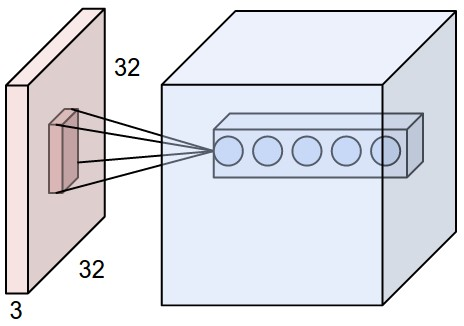
\includegraphics[scale=0.35]{figures/convolution}
	\caption{Illustration\protect\footnotemark ~of the computation of a Convolutional layer. In this example, 5 different filters (in blue) are computed on the original image (in red). Each filter is computed by moving a patch (the small red square) around the input image.}
	\label{fig:convolution}
\end{figure}
\footnotetext{Illustration taken from \url{https://cs231n.github.io/convolutional-networks/}}

A Convolutional layer has some hyperparameters, which determine how the filters are applied to the input.
The main hyperparameters are:
\begin{itemize}
    \item{\textbf{Receptive Field}, which represent the size of the filter. In other words, it determines the dimension of the patch used to compute the filter on the input image. Typical sizes range from 3x3 to 7x7 pixels.
    \item{\textbf{Depth}, which determines the number of filter to be applied. Sometimes this is also called fibre.}
    \item{\textbf{Stride}, which determines the amount of pixel the patch is moved on the image each time. Common values are 1 and 2 pixel.}
}
\end{itemize}
